\documentclass{article}

\usepackage[T1]{fontenc}
\usepackage[utf8]{inputenc}
%\usepackage{ngerman}
\usepackage{amsmath}
\usepackage{graphicx} 
\usepackage[english]{babel}
\usepackage{pdfpages}
\usepackage{geometry} 
\usepackage{float}
\usepackage{subdepth}
\usepackage{hyperref}
\usepackage{siunitx}
\usepackage{listings}
\newcommand{\tabitem}{~~\llap{\textbullet}~~}

\lstset{ 
  backgroundcolor=\color{lightgray}
  }
\title{Resistive Heating in FEniCS\\ \small 
Multiphysics purely based on open-source packages}
\author{Julius Zimmermann}

\begin{document}
\maketitle 
Use the COMSOL tutorial on resistive heating and reproduce it by means of open-source software. 
\section{Geometry: SALOME}
\label{Sec:Geo}
We use \href{http://www.salome-platform.org/}{SALOME} to create the geometry and assign boundaries as depicted in Figs.~\ref{Fig:Geo} and~\ref{Fig:GeoThe}.
The length unit is $\si{m}$.

\begin{figure}[htp]
	 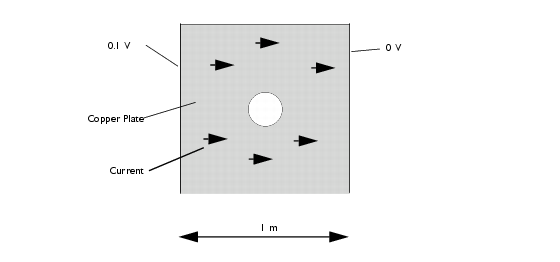
\includegraphics[width=\textwidth]{geometry}
	\caption{Used geometry with electrical boundary conditions.}
		\label{Fig:Geo}
\end{figure}
\begin{figure}[htp]
	 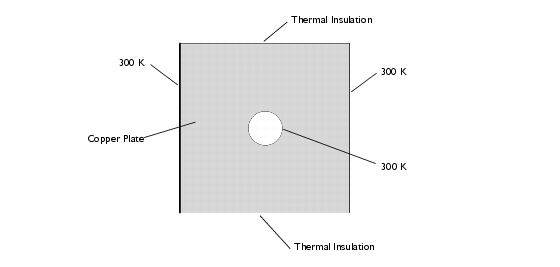
\includegraphics[width=\textwidth]{geometrythermal}
	\caption{Used geometry with thermal boundary conditions.}
		\label{Fig:GeoThe}
\end{figure}

In SALOME, we switch to the \textit{Geometry} module (button adjacent to \textit{new, open} and \textit{save etc.} buttons.
Then we create the geometry following these steps:
\begin{enumerate}
\item click \textit{New Entity} $\rightarrow$ \textit{Primitives} $\rightarrow$ \textit{Rectangle}
\item enter the dimensions: \textit{Height} $=1=$ \textit{Width}
\item click \textit{New Entity} $\rightarrow$ \textit{Primitives} $\rightarrow$ \textit{Disk}
\item enter the radius: $0.1$
\item click \textit{Operations} $\rightarrow$ \textit{Boolean} $\rightarrow$ \textit{Cut}
\item choose \textit{Face\_1} as \textit{Main Object} and \textit{Disk\_1} as \textit{Tool Object}
\end{enumerate}
Having the geometry ready, we assign necessary boundaries. 
Since the plate consists solely of copper, we do not have to specify different domains on the plate.
We only need to distinguish the edges to assign thermal and electrical insulation, respectively as well as the prescribed boundary temperature and voltage.
Hence, we specify different \textit{groups}.
\begin{enumerate}
\item right click \textit{Cut\_1} $\rightarrow$ \textit{Create Group} $\rightarrow$ \textit{Shape Type} (choose the straight line) $\rightarrow$ give a good name such as \textit{insulation\_1} $\rightarrow$ \textit{Select All} and \textit{Remove} the edges you do not need $\rightarrow$ \textit{Apply}
\item repeat this until you have assigned all edges
\end{enumerate}
\section{Mesh: SALOME and GMSH}
\label{Sec:Mesh}
Now we generate a mesh for the geometry created in Sec.~\ref{Sec:Geo}.

Switch to module \textit{Mesh} in SALOME.
\begin{enumerate}
\item click \textit{Mesh} $\rightarrow$ \textit{Create Mesh} $\rightarrow$ choose \textit{Cut\_1} for \textit{Geometry}
$\rightarrow$ \textit{Mesh type} is \textit{triangular} $\rightarrow$  go to \textit{2D} and pick \textit{NETGEN 1D-2D}
\item[!] here we could already set the quality of the mesh by clicking the wheel next to \textit{Hypothesis}. I, for instance, opted for \textit{Fineness} \textit{fine}.
\item \textit{Apply and Close}
\item right click  \textit{Mesh\_1} $\rightarrow$ \textit{Compute}
\item view the mesh, refine, \textit{etc.}
\item use the groups you have created already in the geometry to assign them to the mesh
\item right click \textit{Mesh\_1} and choose \textit{Group on Geometry} and the right type. Then pick the right group from the geometry part and copy paste the name of it. Then click \textit{Apply} for each group and finally \textit{Apply and Close}.
\end{enumerate}
Now we are ready to export the mesh.
Save your model and click \textit{File} $\rightarrow$ \textit{MED file}.
Eventually, \href{http://gmsh.info/}{GMSH} comes into play.
We convert the MED-file to a MSH-file by typing
\begin{lstlisting}[language=bash]
        gmsh "$medfile" -"$dim" -v 0 -o "$mshfile"
\end{lstlisting}
where you have to give the proper name of \lstinline{$medfile}, dimension \lstinline{$dim} and the expected output file \lstinline{$mshfile}.
Now we use \lstinline{dolfin-convert} to obtain an xml-file that is readable by FEniCS
\begin{lstlisting}
        dolfin-convert "$mshfile".msh "$mshfile".xml
\end{lstlisting}
We will then have three files:\\
\lstinline{"$mshfile"_facet_region.xml,"$mshfile"_physical_region.xml,"$mshfile".xml} .
As one goal is to enable multiprocessing, we opt for storing the mesh in the \href{https://en.wikipedia.org/wiki/Hierarchical_Data_Format}{HDF5} format. 
Nevertheless, we could already use xml-files for our FEniCS code.
In order to create a HDF5 file we run:
\begin{lstlisting}
MeshtoHDF5.py "$mshfile"
\end{lstlisting}
with \texttt{MeshtoHDF5.py} being
\begin{lstlisting}
#!/usr/bin/env python

import dolfin as d
import sys

if len(sys.argv) != 2:
    print "specify name of the mesh file (omit .xml)"
    sys.exit(0)

meshname = sys.argv[1]
mesh = d.Mesh(meshname + ".xml")
cd = d.MeshFunction('size_t', mesh, meshname + "_physical_region.xml")
fd = d.MeshFunction('size_t', mesh, meshname + "_facet_region.xml")
hdf = d.HDF5File(mesh.mpi_comm(), meshname + ".h5", "w")
hdf.write(mesh, "/mesh")
hdf.write(cd, "/subdomains")
hdf.write(fd, "/facets")
\end{lstlisting}
If one saves this file in a directory that belongs to the global \texttt{PATH}, it may be called everywhere.
\section{Multiphysics: FEniCS}
\subsection{Theory}
We now use \href{https://fenicsproject.org/}{FEniCS} to solve the multiphysics problem.
In order to do so, we have to formulate the needed equations.
The heat equation for electromagnetic heating reads
\begin{equation}
\label{Eq:HeatEq}
\rho C_p \frac{\partial T}{\partial t} =  \nabla \cdot (k_{\mathrm{iso}} \nabla T) + Q_{\mathrm{e}} \enspace ,
\end{equation}
with the Joule heat
\begin{equation}
Q_\mathrm{e} = \sigma |\nabla V|^2 \enspace .
\end{equation}
To obtain the electric potential $V$, we have to solve the equation
\begin{equation}
\label{Eq:PotEq}
- \nabla \cdot \left(\sigma(\mathbf{r}, T) \nabla V\right) = 0 \enspace .
\end{equation}
We want to consider a temperature-dependent conductivity
\begin{equation}
\sigma (\mathbf{r},T) = \frac{1}{\rho_0 (1+ \alpha ( T(\mathbf{r})- T_0))} \enspace .
\end{equation}

Equations~\eqref{Eq:HeatEq} and~\eqref{Eq:PotEq} have to be transformed to the weak form in order to use them in FEniCS.
Let us start with Eq.~\ref{Eq:HeatEq}. 
First, we take care of the time derivative. 
The finite-difference approach is used to discretise it.
A simple formulation for the $n+1$ time step is
\begin{equation}
\left(\frac{\partial T}{\partial t} \right)^{n+1} \approx \frac{T^{n+1} - T^n}{\varDelta t} \enspace ,
\end{equation}
which is referred to as backward difference (see for instance \href{http://mathworld.wolfram.com/FiniteDifference.html}{here} for other options).
Hence, we end up with 
\begin{equation}
\rho C_p T^{n+1} - k_\mathrm{iso} \varDelta t \Delta T^{n+1} = \rho C_p T^n + \varDelta t \sigma |\nabla V(T^n)|^2  \enspace ,
\end{equation}
where we made use of the fact that $k_\mathrm{iso}$ is not position-dependent.
For deriving the weak formulation we start with
\begin{equation}
\intop_\Omega \left( \rho C_p T^{n+1} - k_\mathrm{iso} \varDelta t \Delta T^{n+1} \right) v \mathrm{d}\Omega	 = \intop_\Omega \left(\rho C_p T^n + \varDelta t \sigma |\nabla V(T^n)|^2\right) v \mathrm{d}\Omega	\enspace ,
\end{equation}
where $v$ are the test functions.
We do not touch the right-hand side (RHS) and focus on the left-hand side (LHS).
Integration by parts yields
\begin{equation}
\intop_\Omega \left( \rho C_p T^{n+1} - k_\mathrm{iso} \varDelta t \Delta T^{n+1} \right) v \mathrm{d}\Omega = \intop_\Omega \left( \rho C_p T^{n+1} v + k_\mathrm{iso} \varDelta t \nabla T^{n+1} \nabla v\right)  \mathrm{d}\Omega + \intop_{\partial \Omega}  k_\mathrm{iso} \varDelta t (\nabla T^{n+1} \cdot \mathbf{n}) v \mathrm{d}s \enspace ,
\end{equation}
where $\mathbf{n}$ is the normal vector on the boundary and $\nabla T^{n+1} \cdot \mathbf{n}$ is often written as $\frac{\partial T^{n+1}}{\partial n}$ .
The term on the boundary vanishes for Dirichlet boundary conditions since the test functions are zero there. 
However, for Neumann boundaries (as the thermally and electrically insulated sides of our geometry) we have to keep this term. 
Nevertheless, we consider $\frac{\partial T^{n+1}}{\partial n}= 0$ and $\frac{\partial V}{\partial n}=0$ and can thus drop this term, too.
Eventually, the problem reads
\begin{equation}
\label{Eq:WeakT}
 \intop_\Omega \left( \rho C_p T^{n+1} v + k_\mathrm{iso} \varDelta t \nabla T^{n+1} \nabla v\right)  \mathrm{d}\Omega  = \intop_\Omega \left(\rho C_p T^n + \varDelta t \sigma |\nabla V(T^n)|^2\right) v \mathrm{d}\Omega	\enspace .
\end{equation}
For the Eq.~\eqref{Eq:PotEq} we can perform similar steps and end up with
\begin{equation}
\label{Eq:WeakPot}
\intop_\Omega \sigma(\mathbf{r}, T) \nabla V \nabla v \mathrm{d}\Omega = \intop_\Omega f v \mathrm{d} \Omega,~~~ f=0
\end{equation}
\subsection{Implementation}
\subsubsection{General header}
I use the python interface for FEniCS.
Therefore, I load 
\begin{lstlisting}
import dolfin as d
import matplotlib.pyplot as plt
\end{lstlisting}
\textit{Dolfin} contains all functions we need and \textit{pyplot} is a nice tool for plotting.
\subsubsection{Loading the mesh}
I have saved the mesh in a file, that is in the directory \texttt{Mesh}. 
There, I also have a refined mesh with $4795$ DOFs, which comes close to the COMSOL reference. 
I load them as well as the facets (needed for the boundaries) and the physical regions (could be used to assign material parameters, here not needed). 
Eventually, I have a look at the mesh to check if it is loaded properly.
\begin{lstlisting}
meshpath = '../Mesh/'
if len(sys.argv) > 1:
    meshname = sys.argv[1]
else:
    meshname = 'MeshDiskwithHoleAuto'
mesh_file = meshpath + meshname + '.h5'
if not os.path.isfile(mesh_file):
    print("Specify correct name for meshfile!")
    sys.exit(0)
mesh = d.Mesh()
hdf = d.HDF5File(mesh.mpi_comm(), mesh_file, "r")
hdf.read(mesh, "/mesh", False)
cells = d.MeshFunction("size_t", mesh)
hdf.read(cells, "/subdomains")
facets = d.MeshFunction("size_t", mesh)
hdf.read(facets, "/facets")
d.plot(mesh)
plt.show()
\end{lstlisting}
I also declare a datafile to save the simulation results.
One is in HDF5 format, one in plain ASCII text format.
The latter does not work if MPI is used.
\begin{lstlisting}
datafileHDF5 = d.HDF5File(mesh.mpi_comm(), "TemperatureDevelopment_test.h5", "w")
datafile = open('TemperatureDevelopment_test.dat', 'w')
\end{lstlisting}
\subsubsection{Parameter declaration}
The used physical properties for Eqs.~\eqref{Eq:HeatEq} and~\eqref{Eq:PotEq} are given in Tab.~\ref{tab:1}.
We have to write them down in a python script for FEniCS and use the command \textit{Constant} of the \textit{dolfin}-class:
\begin{lstlisting}
T_0 = d.Constant(300.)
T_ref = d.Constant(293.)
V0 = d.Constant(.1)  # set boundary value of electrode to 10 V
f = d.Constant(0.0)
rho_0 = d.Constant(1.754e-8)  # reference resistivity
C_p = d.Constant(340.)  # heat capacity
rho = d.Constant(8930.)  # density  [kg/m^3]
k_iso = d.Constant(384.)  # thermal conductivity [W/(m*K)]
alpha = d.Constant(3.9e-3)  # T-dependent resistivity coeff. [1/K]

t_max = 2000.  # time in s
dt = 50.  # time step
num_steps = int(t_max / dt)
\end{lstlisting}
The parameters for the time-stepping algorithm are not declared as FEniCS constants since they are not passed to it.
The temperature-dependent resistivity is implemented as a python-function with \textit{Temp} being supposed to be the temperature resulting from the FEniCS calculation:
\begin{lstlisting}
# temperature-dependent resistivity
def sigma_T(Temp):
    return 1. / (rho_0 * (1. + alpha * (Temp - T_0)))
\end{lstlisting}
\begin{table}[!htp]
\caption{Physical properties for simulating Joule heating.}
\label{tab:1} 
\begin{center}
\begin{tabular}{l@{\hskip 8pt}l@{\hskip 8pt}}
\hline\noalign{\smallskip}
parameter & value  \\
\noalign{\smallskip}\hline\noalign{\smallskip}
$\rho_0$& $\SI{1.754e-8}{\ohm}$\\
$C_p$ & $\SI{340}{\J\per\kg\per \K}$\\
$\epsilon_r$ & $1$ \\
$\rho$ & $\SI{8940}{\kg \per \m^3}$\\
$k_{\mathrm{iso}}$ & $\SI{400}{\W\per\m\per\K}$\\
$\alpha$ & $\SI{3.862e-3}{\per\K}$\\
$T_\mathrm{ref}$ & $\SI{293.15}{\K}$\\
\noalign{\smallskip}\hline
\end{tabular}
\end{center}
\end{table}

\subsubsection{Boundary conditions and initial condition}
We need to declare a function space.
We use 2\textsuperscript{nd} order Lagrange-elements (see \href{https://fenicsproject.org/olddocs/dolfin/1.4.0/python/programmers-reference/functions/functionspace/FunctionSpace.html}{FEniCS documentation} for other options).
\begin{lstlisting}
# declare function space
V = d.FunctionSpace(mesh, 'CG', 2)
print("Number of DOFs: {}".format(V.dim()))
dx = d.dx
\end{lstlisting}
The number of DOFs is printed here and can be compared to COMSOL (there it is $4548$).
For this function space, we impose boundary and initial conditions. 
We use the facets defined in GMSH.
To get the numbering of them, you may have a look at the \textit{.msh}-file.
We have
\begin{lstlisting}
'''
GMSH boundaries (from .geo or .msh file)
The number on the left denotes:
1 stands for Physical Line, 
2 stands for Physical Surface, 
3 stands for Physical Volume
(nomenclature taken from Computational Reality book of Abali)
use the auto file!

1 1 "Insulation_1"
1 2 "Insulation_2"
1 3 "Boundary_1"
1 4 "Boundary_2"
1 5 "CircleCenter"
2 6 "Copper"
'''
\end{lstlisting}
Therefore, we arrive at:
\begin{lstlisting}
# boundary conditions
# see declaration from GMSH above
# Dirichlet for assigned electric potential
bc0_e = d.DirichletBC(V, V0, facets, 3)
bc1_e = d.DirichletBC(V, f, facets, 4)

# Dirichlet for assigned temperature
bc0_t = d.DirichletBC(V, T_0, facets, 3)
bc1_t = d.DirichletBC(V, T_0, facets, 4)
bc2_t = d.DirichletBC(V, T_0, facets, 5)  # circle

bc_e = [bc0_e, bc1_e]
bc_t = [bc0_t, bc1_t, bc2_t]
\end{lstlisting}
The initial value for the temperature is $T_\mathrm{ref}$.
The \textit{interpolate} function projects the value to the whole domain of our function space.
\begin{lstlisting}
# Define initial value, which will later
# be the solution from the previous (n-th) time step
T_n = d.Function(V)
T_n = d.interpolate(T_ref, V)
\end{lstlisting}
\subsubsection{Solving the PDE}
Now, we finally implement Eqs.~\eqref{Eq:WeakT} and~\eqref{Eq:WeakPot}. Note, that the electric potential is called \textit{psi} in the code. \textit{T\_n1} refers to T$^{n+1}$.
\begin{lstlisting}
# Define variational problem for temperature and potential
psi = d.TrialFunction(V)  # trial for potential
T_n1 = d.TrialFunction(V)  # trial for temperature
v = d.TestFunction(V)
# potential 
a = d.inner(sigma_T(T_n) * d.grad(psi), d.grad(v)) * dx
L = f * v * dx  # keep in mind: f=0

psi = d.Function(V)  # solution for potential
# temperature
a_1 = (rho * C_p * T_n1 * v * dx
       + k_iso * dt * d.dot(d.grad(T_n1), d.grad(v)) * dx)
L_1 = (rho * C_p * T_n
       + dt * sigma_T(T_n) * d.dot(d.grad(psi), d.grad(psi))) * v * dx
T_n1 = d.Function(V)  # solution for T
\end{lstlisting}

While stepping forward in time, we solve for the potential, use it to calculate the Joule heat and obtain a solution for the temperature. 
The solution is assigned to the temperature of the previous timestep, T\textsuperscript{n}.
We store the simulation results at each time step as:
\begin{itemize}
\item temperature at $(0.0, 0.25)$ (plain ASCII)
\item temperature distribution on whole domain as HDF5 and as PVD (ParaView) file. These two data types can be readily used in multiprocessing, too.
\end{itemize}
\begin{lstlisting}
# Time-stepping
t = 0
# write temperature at (0., 0.25) to file
datafile = open('TemperatureDevelopment.dat', 'w')
# write initial temperature
datafile.write("%f\t%f\n" % (t, T_n(d.Point(0., 0.25))))
datafileHDF5.write(T_n, "/T_0")
# open ParaView file and write initial T
file = d.File('JouleHeatingT.pvd')
file << T_n

for n in range(num_steps):
    # solve EM problem
    d.solve(a == L, psi, bc_e)
    # p = d.plot(psi)
    # plt.colorbar(p)
    # plt.show()
    # Update current time
    t += dt
    # Compute solution
    d.solve(a_1 == L_1, T_n1, bc_t)
    # d.plot(T_n)
    # plt.colorbar(p)
    # plt.show()
    # Update previous solution
    T_n.assign(T_n1)
    # evaluate temperature at point of interest
    datafile.write("%f\t%f\n" % (t, T_n(d.Point(0., 0.25))))
        datafileHDF5.write(T_n, "/T_{}".format(n + 1))
    file << T_n
datafile.close()
# plot final solution
p = d.plot(T_n1)
plt.colorbar(p, format='%3.3f')
# compute heat flux on vector function space
W = d.VectorFunctionSpace(mesh, 'Lagrange', 1)
hflux = d.project(-k_iso * d.grad(T_n), W)
d.plot(hflux, mode="glyphs", color="white")
save to file
plt.savefig("TemperatureFlux.png")
plt.show()
\end{lstlisting}
The resulting temperature and flux can be seen in Fig.~\ref{Fig:TempFlux}.
The plot command does not work in parallel mode.
Thus, I have added a description for post-processing in Sec.~\ref{Sec:PostProc}.
\subsection{Results}
The temperature distribution and the flux look very much as obtained by means of COMSOL.

To compare COMSOL and FEniCS, the temperature is evaluated at a certain point for each time step.
Since the geometries are shifted by$(0.5, 0,5)$, this point is $(0.5, 0.75)$ in COMSOL and $(0.0, 0.25)$ in FEniCS.
Figure~\ref{Fig:TempTimeComsFen} shows that the result does not converge to the same value.
The difference equals $\approx \SI{1.3}{K}$. 
To clarify, why that happens, one has to check some things. Do the studies fully coincide (choice of paramters etc.), which elements and method of evaluating the temperature have been used, etc.?
The mesh could also play a role, but a minor one. 
For instance, a rough mesh with only 550 DOF yields a final temperature that is $\SI{0.2}{K}$ off from the solution with $>4000$ DOFs. 
\begin{figure}[H]
\label{Fig:TempFlux}
\centering
\includegraphics[width=\textwidth]{FenicsStudy/TemperatureFlux}
\caption{Temperature and Flux plotted with FEniCS. To obtain the same picture as with COMSOL, the usage of \href{https://www.paraview.org/}{Paraview} might be necessary.}
\end{figure}
\begin{figure}[H]
\label{Fig:TempTimeComsFen}
\centering
\includegraphics[width=\textwidth]{FenicsStudy/compareTemps}
\caption{Temperature at a certain point. Comparison of COMSOL and FEniCS results.}
\end{figure}
\section{Automatising the whole approach}
Use the notebook section in SALOME. 
Then dump python file, here it is called \textit{MeshwithHoleAutomatised.py}.

To automatise the approach, a script called \textit{solve\_automated.sh} is prepared.
It follows all the steps originally done by hand.
The meshname is provided as an input to the python code.
\begin{lstlisting}
# !/bin/bash
# name of study
FENICS='JouleHeating'
# parameters for rectangle and circle
h=1
w=1
r='0.1'
# meshname
mn='MeshDiskwithHole_test'

# change mesh parameters in SALOME file
cd Mesh
SALOME = 'MeshwithHoleAutomatised'
# run SALOME with arguments: meshname, height, width, radius
salome -t "$SALOME".py args:$mn,$h,$w,$r
# convert to MSH
MED2MSH.sh "$mn".med 2
# convert to XML
MSH2XML.sh "$mn".msh
# convert to HDF5
MeshtoHDF5.py "$mn" 


# go to Fenics folder and run study
cd ../FenicsStudy
python $FENICS.py $mn
\end{lstlisting}
\section{Postprocessing}
\label{Sec:PostProc}
\subsection{Paraview}
\href{https://www.paraview.org/}{ParaView} is an awesome software package to visualize the simulation results.
It also offers the possibility to export python scripts.
Open ParaView and load the \texttt{pvd}-file that was generated during the simulation.
Click \textit{Apply} to see the result.
One could also choose a single \texttt{vtu}-file belonging to a particular time step.
 
We would like to create an animation.
Thus, we change the color bar a little.
Click \textit{View} $\rightarrow$ \textit{Color Map Editor}.
In the dialogue on the right hand side open the window \textit{Edit Color Legend Parameters}.
Change the title and the label format accordingly.

Now rescale to custom range ($\SI{293}{\K} .. \SI{390}{\K}$).
We also add a contour with a temperature range of $\SI{310}{\K} .. \SI{390}{\K}$ with a $\SI{10}{\K}$ step.
The time is shown in the final graphic by adding \textit{Filters} $\rightarrow$ \textit{Annotation} $\rightarrow$ \textit{Annotate Time Filter}.

We can export the study to a python script by saving the state.
After adding to the python script the following lines
\begin{lstlisting}
AnimateReader(jouleHeatingTpvd, filename='movie.png')
\end{lstlisting}
we obtain a number of png-files which we can convert to a gif by
\begin{lstlisting}
convert -delay 20 -loop 0 movie.*.png movie.gif
\end{lstlisting}
\subsection{FEniCS}
During an run in parallel mode, evaluation of functions at certain points, plotting etc. should be avoided.
Thus, one can also use FEniCS and some python tools for postprocessing
\begin{lstlisting}
import dolfin as d
import sys
import os
import numpy as np
import matplotlib.pyplot as plt
    
meshpath = '../Mesh/'
if len(sys.argv) > 1:
    meshname = sys.argv[1]
else:
    meshname = 'MeshDiskwithHoleAuto'
    meshname = meshname + "_refined"
mesh_file = meshpath + meshname + '.h5'
if not os.path.isfile(mesh_file):
    print("Specify correct name for meshfile!")
    sys.exit(0)
mesh = d.Mesh()
hdf = d.HDF5File(mesh.mpi_comm(), mesh_file, "r")
datafile = d.HDF5File(mesh.mpi_comm(), "TemperatureDevelopment_test.h5", "r")
hdf.read(mesh, "/mesh", False)
\end{lstlisting}
First, we load the mesh and the datafile.
Then, we can continue with extracting data or plotting it
\begin{lstlisting}
t_max = 2000.  # time in s
dt = 50.  # time step
num_steps = int(t_max / dt)
k_iso = d.Constant(384.)
    
V = d.FunctionSpace(mesh, 'CG', 2)
T_n = d.Function(V)
T_dev = np.array([])
for n in range(num_steps + 1):
    datafile.read(T_n, "/T_{}".format(n))
    T_dev = np.append(T_dev, T_n(d.Point(0., 0.25)))

data = np.loadtxt('TemperatureDevelopmentCOMSOL.dat', dtype=float, comments='%')
plt.ylim((293, 375))
plt.xlim((0, 2050))
plt.ylabel('T[K]')
plt.xlabel('t [s]')
plt.plot(dt * np.arange(0, num_steps + 1), T_dev, label='FEniCS')
plt.plot(data[:, 0], data[:, 1], label='COMSOL')
plt.legend(loc="upper left") 
plt.show()

W = d.VectorFunctionSpace(mesh, 'Lagrange', 1)
hflux = d.project(-k_iso * d.grad(T_n), W)
p = d.plot(T_n)
plt.colorbar(p, format='%3.1f')
d.plot(hflux, mode="glyphs", color="white")
plt.savefig("TemperatureFlux_test.png")
plt.show()
\end{lstlisting}
\section{Literature overview}
I highly recommend the book of Abali~\cite{Abali2017}. 
He gives many examples how FEniCS can be used for multiphysics simulations.
For some examples of how to use FEniCS have a look at the \href{https://fenicsproject.org/pub/tutorial/html/ftut1.html}{Fenics Tutorial} or the Fenics book~\cite{LoggMardalEtAl2012a}.
A book that focusses on many important things but only features the C++ interface is given in Ref.~\cite{vabishchevich2015computational}.
\bibliographystyle{abbrv}
\bibliography{authorref}
\end{document}


